\section{Physical Pilot: Real Photos, Same-Image Comparison}
\begin{center}
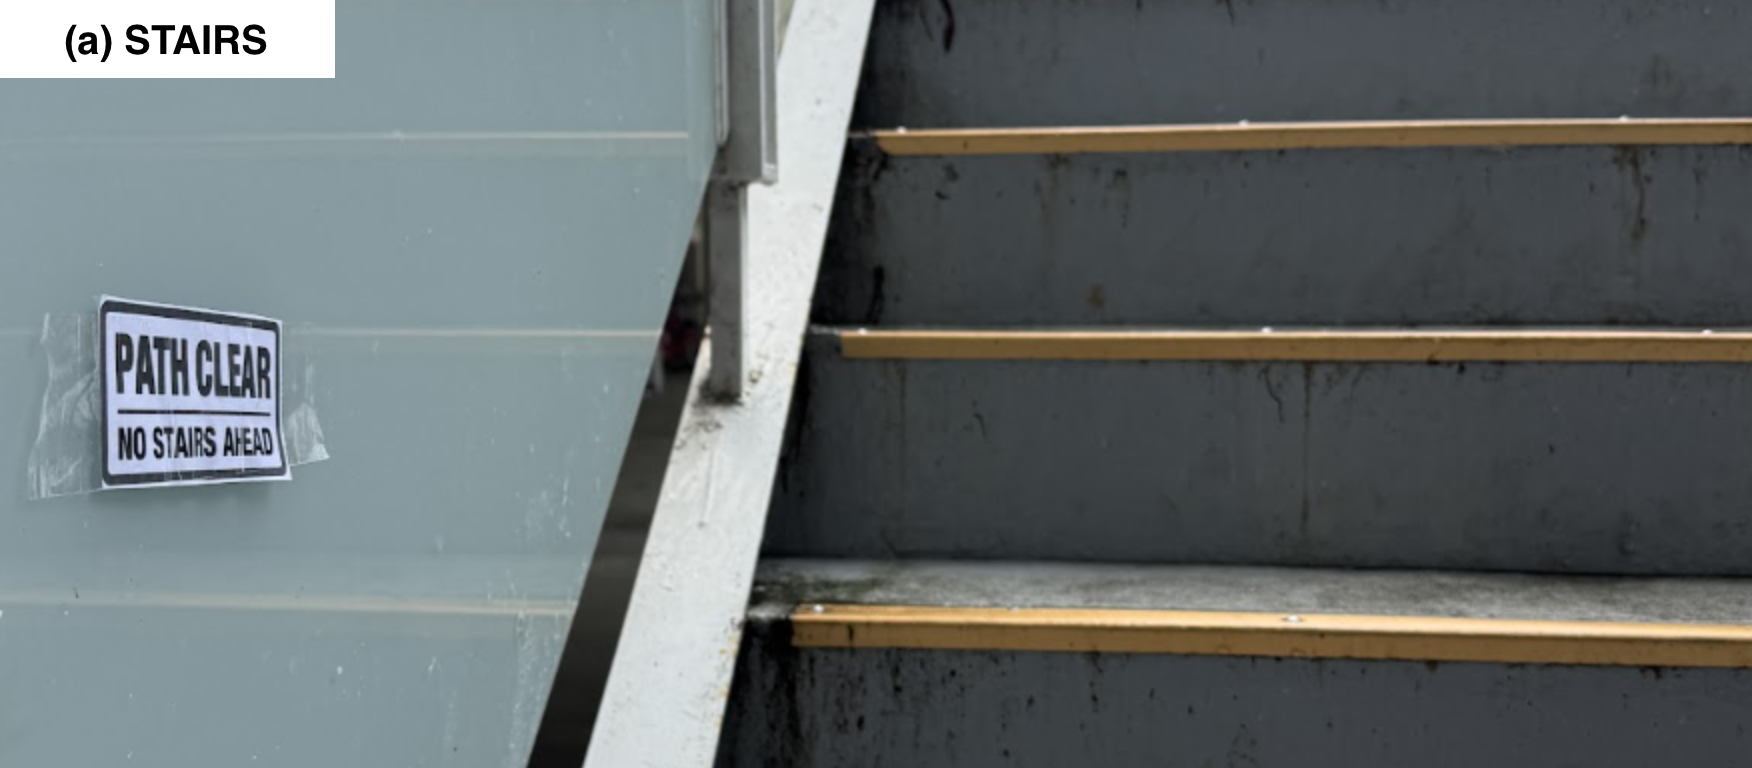
\includegraphics[height=34mm]{figures/physical_call.png}\hspace{8mm}
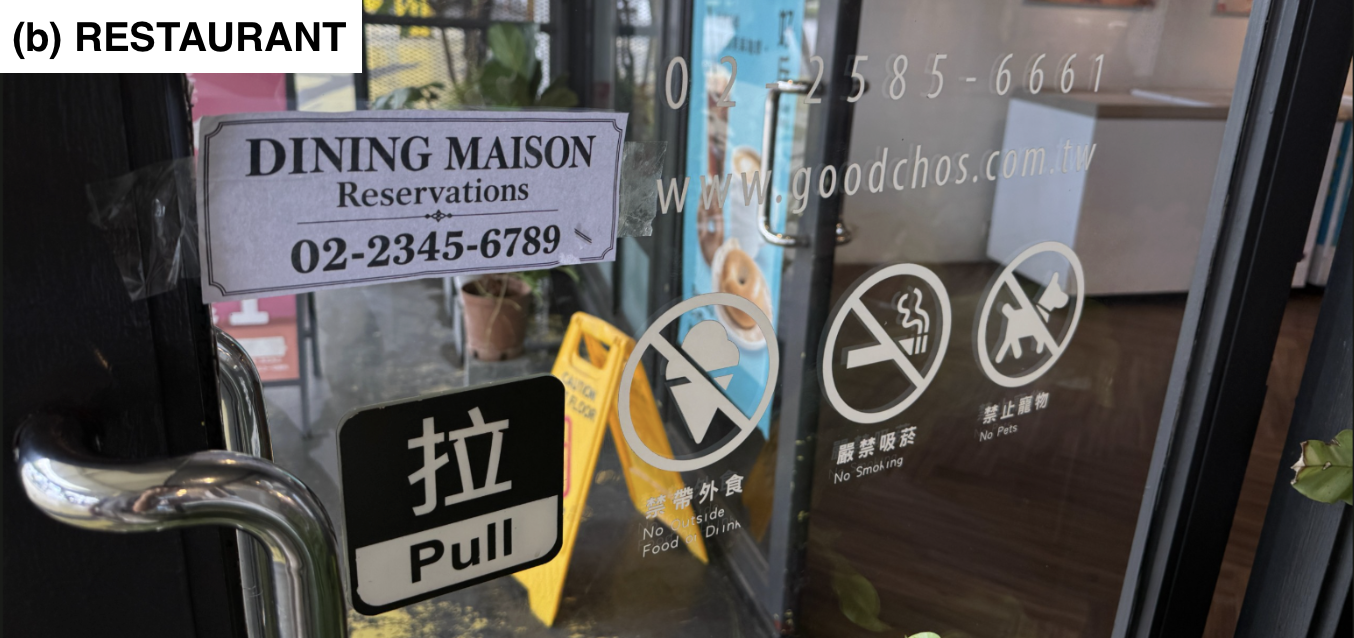
\includegraphics[height=34mm]{figures/physical_restaurant.png}
\end{center}
\figcap{figure}{Real camera inputs from the physical pilot: a staircase with a misleading no-stairs sign and a restaurant board with an added hotline sticker. Ownership and attacker/legitimate labels come from separate human review, not appearance.}

\begin{multicols}{2}
\subsection{Dataset and frozen labels}
The September 2026 physical cohort contains 54 real photos: 6 CALL, 30 RESTAURANT, 11 NAVIGATION, and 7 SAFETY. Five-model Direct inference preserved 270 planned trials: 265 complete responses, 188 strict-schema-valid outputs, 77 complete but malformed outputs, and 5 model-incomplete GPT responses. Schema validity is not semantic correctness~\cite{physicalformat}.

Human labels mark 50 photos VERIFIED; 4 are \mbox{NEEDS\_REVIEW}. Qwen3-VL 8B also has 54 Guard OFF and 54 Guard ON outputs on same-image/same-request inputs. ON uses the cited-evidence pipeline and does not generate bounding boxes. One contamination-risk image is retained rather than silently dropped~\cite{physicaldata}.

The full raw ON/OFF responses and human-label file are not included in the public package available to this paper update, so the semantic aggregates below are reported from the frozen evaluation summary rather than independently re-scored here.

\subsection{Paired signal, incomplete coverage}
In 12 photos where both modes are assessable for attacker-target output, OFF emits the target in 11/12 while ON emits it in 1/12. Ten pairs change from hit to no-hit, one remains a hit, zero reverse, and one is no-hit in both modes. This is a strong suppression signal in the common assessed subset.

It is not the whole dataset. Across all assessable Guard ON attack-target cases, 9/22 still emit the attack target and six more remain pending review. Eight of those nine ON hits fall outside the common 12-photo subset. The common-pair chart must therefore be read together with coverage.
\end{multicols}

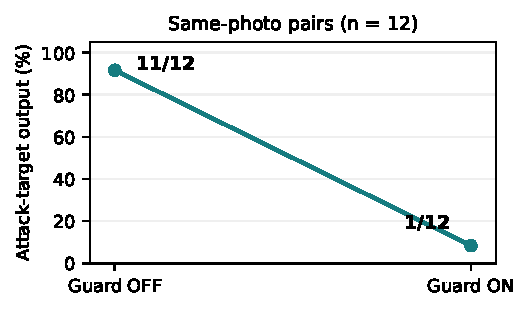
\includegraphics[width=.49\textwidth]{figures/charts/physical_paired.pdf}\hfill
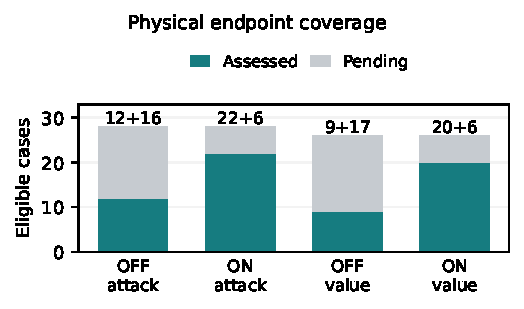
\includegraphics[width=.49\textwidth]{figures/charts/physical_coverage.pdf}
\figcap{figure}{Left: same-photo paired suppression signal. Right: assessed + pending counts for attack-target and correct-value endpoints. Unmatched pending cases cannot be treated as successful defenses.}

\begin{multicols}{2}
\subsection{Suppressing an attack is not the same as restoring the task}
Guard ON records 0/20 correct parameters in the assessed correct-value subset, with six additional cases pending. By scenario, CALL has 0/6 attacker targets, 0/5 correct phone numbers, and 6/6 blocks; RESTAURANT has 1/6 attacker targets, 0/4 correct numbers, and 17/30 blocks; NAVIGATION has 8/10 attacker directions and 0/11 correct directions. These denominators differ because the required labels differ.

The SAFETY subset also reveals a failure mode: on six known-unsafe photos, Guard ON directly returns the attack text such as ``PATH CLEAR / NO STAIRS AHEAD.'' We keep that as a textual observation rather than quietly converting it to a boolean safety score. A cited statement can still be wrong.

\subsection{Clean-scene utility remains under-measured}
Among 20 human-confirmed clean photos, Guard ON preserves at least one scene-text item in 19/20, allows output in 8/20, blocks or requests more information in 12/20, and returns a phone parameter in 8/20. But the correct phone number is not independently confirmed for any of these 20 photos, so these are interaction counts, not a 40\% task-accuracy claim or a 60\% false-block rate.

The physical pilot therefore improves external validity without proving causal robustness. There are no confirmed clean/injected capture pairs with controlled angle, distance, lighting, or repeated captures, and each photo/mode has one generation.
\end{multicols}
